\documentclass{beamer}

\usetheme{Madrid}

\usepackage{lipsum}
\usepackage{multicol}
\usepackage{listings}


% Define a custom color
\definecolor{backcolour}{rgb}{255,255,255}
\definecolor{codegreen}{rgb}{0,0.6,0}

% Define a custom style
\lstdefinestyle{myStyle}{
    backgroundcolor = \color{backcolour},   
    commentstyle = \color{codegreen},
    basicstyle=\linespread{0.4}\tiny,
    breakatwhitespace=false,         
    breaklines=true,        
    keepspaces=true,                               
    showspaces=false,                
    showstringspaces=false,
    showtabs=false,                  
    tabsize=2,
}

% Use \lstset to make myStyle the global default
\lstset{style=myStyle}

\usepackage{graphicx}
\usepackage{listings}
\usepackage{verbatim}
\linespread{1.5}
\usepackage{pgfplots}
\usepackage{tikz}

\usepackage{amsmath, amsthm, amssymb, latexsym}

%\newtheorem{definition}{Definition}

\newcommand{\pathtoimages}{/Users/charlesrambo/Desktop/Bootcamp24/Images}

\title{Unit 1: Calculus}
\author{Charles Rambo}
\institute{UCLA Anderson}
\date{2024}


\begin{document}
\input{systempreamble}


\frame{\titlepage}

\begin{frame}[allowframebreaks]

\frametitle{Table of Contents}
\tableofcontents
\end{frame}

\section{Limits}

\begin{frame}
\begin{center}
\Huge Limits
\end{center}
\end{frame}

\frame{
\frametitle{Definition}

\begin{Definition}
{
\linespread{1}
\begin{enumerate}
\item[(a)] Define $\displaystyle\lim_{x\to a} f(x) = L$ to mean for all $\epsilon > 0$ there exists a $\delta > 0$ such that
$$
0 < |x - a| < \delta\qquad\text{implies}\qquad \left|f(x) - L\right| <\epsilon.
$$
\item[(b)] Define $\displaystyle\lim_{x\to \infty} f(x) = L$ to mean for all $\epsilon > 0$ there exists an $N$ such that
$$
x \geq N \qquad\text{implies}\qquad \left|f(x) - L\right| <\epsilon.
$$
\item[(c)] Define $\displaystyle\lim_{x\to -\infty} f(x) = L$ to mean 
for all $\epsilon > 0$ there exists an $N$ such that
$$
x \leq N \qquad\text{implies}\qquad \left|f(x) - L\right| <\epsilon.
$$
\end{enumerate}
}
\end{Definition}
}

\begin{frame}
\frametitle{$\displaystyle\lim_{x\to a} f(x) = L$}

\begin{figure}
\begin{tikzpicture}[scale = 2.5]

\draw[->] (-0.1, 0) -- (2, 0) node[right] {$x$};
\draw[->] (0, -0.1) -- (0, 2) node[above] {$y$};

 \draw[->, domain=0:2, smooth, variable= \x, blue] plot ({\x}, {sqrt(\x)});
 
 \draw[fill=white] (1, 1) circle (1pt);
 
  \draw[fill=black] (1, 1.5) circle (1pt);
 
\draw[style=dashed] (2, 1.2) -- (-0.1, 1.2) node[left] {$L + \epsilon$};
\draw[style=dashed] (2, 0.8) -- (-0.1, 0.8) node[left] {$L - \epsilon$};
\draw (0.08, 1) -- (-0.08, 1) node[left] {$L$};

\draw[style=dashed] (0.7, 2) -- (0.7, -0.1) node[below] {$a - \delta$};
\draw[style=dashed] (1.3, 2) -- (1.3, -0.1) node[below] {$a + \delta$};

\draw (1, 0.08) -- (1, -0.08) node[below] {$a$};

\end{tikzpicture}
\end{figure}

\end{frame}

\begin{frame}
\frametitle{$\displaystyle\lim_{x\to \infty} f(x) = L$}

\begin{figure}
\begin{tikzpicture}[scale = 2]

\draw[->] (-0.1, 0) -- (5, 0) node[right] {$x$};
\draw[->] (0, -0.1) -- (0, 2) node[above] {$y$};

 \draw[->, domain=0:5, samples=500, variable= \x, blue] plot ({\x}, {0.7 * sin(500 * \x)/(1.5 * \x + 0.5) + 1});
 
 
\draw[style=dashed] (5, 1.2) -- (-0.1, 1.2) node[left] {$L + \epsilon$};
\draw[style=dashed] (5, 0.8) -- (-0.1, 0.8) node[left] {$L - \epsilon$};
\draw (0.08, 1) -- (-0.08, 1) node[left] {$L$};


\draw[style=dashed] (2.1, 2) -- (2.1, -0.1) node[below] {$N$};
\draw (2.1, 0.08) -- (2.1, -0.08);


\end{tikzpicture}
\end{figure}

\end{frame}



\begin{frame}[t]
\frametitle{Using the Definition}
\begin{Example}
Prove
$$
\displaystyle\lim_{x\to\infty} \frac{1}{x^p} = 0
$$
for all $p > 0$.
\end{Example}
\end{frame}

\begin{frame}
\frametitle{$\epsilon$-$\delta$ Limit Definition on YouTube}
Watch BlackPenRedPen explain the $\epsilon$-$\delta$ limit definition {\tiny(\url{https://www.youtube.com/watch?v=DdtEQk_DHQs})}. There's another video where he goes over the $x\to\infty$ case {\tiny(\url{https://youtu.be/9JMFLzHtljA?si=1WPW-fmaf2DBe3Ph})}.
\begin{center}

\includegraphics[scale = 0.20]{\pathtoimages/blackpenredpen.png}
\end{center}
\end{frame}

\frame{
\frametitle{Properties of Limits}
\begin{Theorem} 
Suppose $a$ is in the interval $[-\infty, \infty]$. Let
$$
\lim_{x\to a} f(x) = L_1\qquad\text{and}\qquad\lim_{x\to a} g(x) = L_2.
$$
\begin{enumerate}
\item[(a)] $\displaystyle\lim_{x\to a} \alpha f(x) + \beta g(x) = \alpha L_1 + \beta L_2$ for any real constants $\alpha$ and $\beta$
\item[(b)] $\displaystyle\lim_{x\to a} f(x) \cdot g(x) = L_1\cdot L_2$
\item[(c)] $\displaystyle\lim_{x\to a} \frac{1}{f(x)} = \frac{1}{L_1}$ if $L_1 \neq 0$.
\end{enumerate}
\end{Theorem}
}

\begin{frame}
\frametitle{Useful Limits}
\begin{Theorem}
Suppose $p > 0$.
\begin{enumerate}
\item[(a)] $\displaystyle\lim_{x\to\infty} \frac{1}{x^p} = 0$
\item[(b)] $\displaystyle\lim_{x\to\infty} p^{1/x} = 1$
\item[(c)] $\displaystyle\lim_{x\to\infty} x^{1/x} = 1$
\item[(d)] If $ a > 0$, $\displaystyle\lim_{x\to 0} \frac{a^x - 1}{x} = \ln a$
\item[(e)] If $|r| < 1$, then $\displaystyle\lim_{x\to\infty} r^x = 0$
\end{enumerate}
\end{Theorem}
\end{frame}

\begin{frame}[t]
\frametitle{Python Example}
\begin{Example}
Define
$$
f(x) = \begin{cases} 
\sin\left(\frac{1}{x}\right),	&	x\neq 0\\ 0,	&	x = 0.
\end{cases}
$$
Graph $f$ in Python to see that $\displaystyle\lim_{x\to 0} f(x)$ does not exist.
\end{Example}
\end{frame}

\begin{frame}[fragile]
\frametitle{Python Example Cont.}

\begin{lstlisting}[language=Python]
# Import modules 
import numpy as np
import matplotlib.pyplot as plt

# Use latex
plt.rcParams['text.usetex'] = True

# Use Seaborn style
plt.style.use('seaborn')

# Define f
f = lambda x: 0 if x == 0 else np.sin(1/x)   
        
# Let's graph on the interval [-pi, pi]
x_vals = np.arange(-np.pi, np.pi, np.pi/200)

# Calculate the y-values
y_vals = [f(x) for x in x_vals]

# Generate the plot
plt.plot(x_vals, y_vals)

# Label the x-axis
plt.xlabel(r'$x$')

# Label the y-axis
plt.ylabel(r'$y$')

# Give the graph a title
plt.title(r'Graph of $y = f(x)$')

# Save the figure
plt.savefig(path + r'Images/ex1-1.png')

# Display the plot
plt.show()

\end{lstlisting}
\end{frame}

\begin{frame}
\frametitle{Python Example Result}
The graph isn't perfect, but it's enough to see that $f$ doesn't approach anything in particular as $x$ approaches 0.

\begin{center}
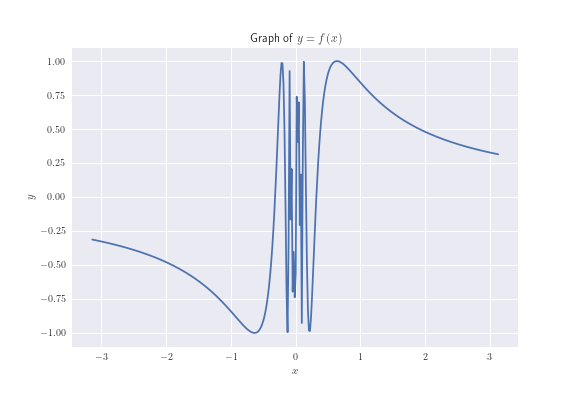
\includegraphics[scale = 0.4]{\pathtoimages/ex1-1.png}
\end{center}
\end{frame}


\section{Continuity} 

\begin{frame}
\begin{center}
\Huge Continuity
\end{center}
\end{frame}

\begin{frame}
\frametitle{Continuity}
\begin{Definition}
\begin{enumerate}
\item[(a)] A function $f$ is continuous at $a$ if $\displaystyle \lim_{x\to a} f(x) = f(a)$.
\item[(b)] A function $f$ is continuous on the set $A$ if
$$
a\in A\qquad\text{implies}\qquad \lim_{x\to a} f(x) = f(a).
$$
\end{enumerate}
\end{Definition}
\end{frame}

\begin{frame}
\frametitle{Continuity Idea}
Continuous functions have no breaks, i.e. if you were to draw them you would never need to lift your pencil. 
\begin{center}
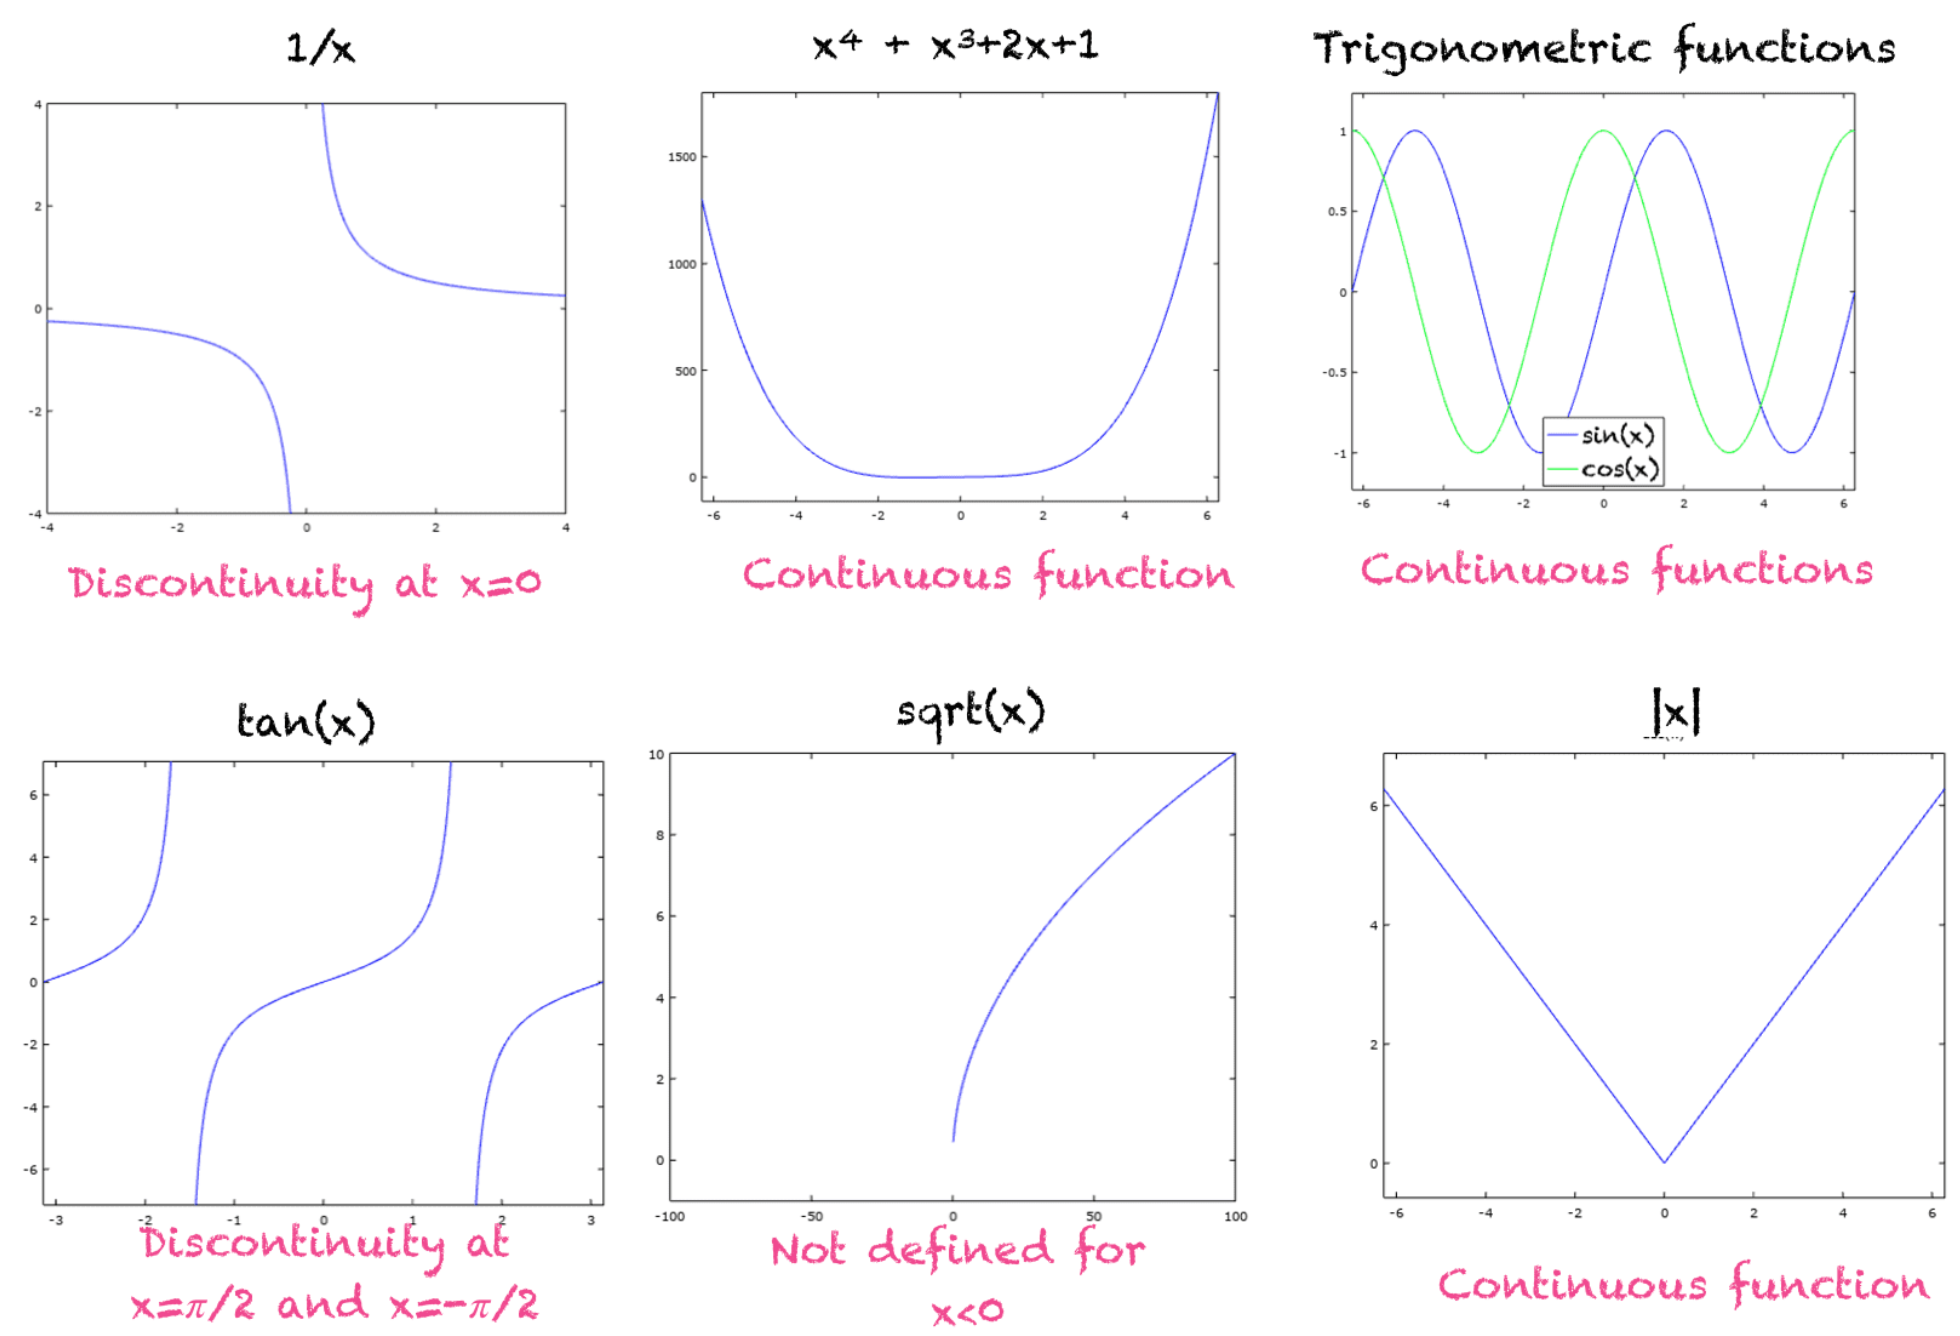
\includegraphics[scale = 0.2]{\pathtoimages/cont.png}
\end{center}
\tiny\url{https://machinelearningmastery.com/continuous-functions/}
\end{frame}

\begin{frame}
\frametitle{Useful Theorem}
\begin{Theorem}
If $f$ is continuous at $b$ and $\displaystyle\lim_{x\to a} g(x) = b$, then
$$
\lim_{x\to a} f\Big(g(x)\Big) = f\left(\lim_{x\to a} g(x)\right) = f(b).
$$
\end{Theorem}
\end{frame}

\begin{frame}[t]
\frametitle{Example}
\begin{Example}
Suppose $p > 0$. Compute $\displaystyle\lim_{x\to\infty} p^{1/x}$.
\end{Example}
\end{frame}


\section{Derivatives} 

\begin{frame}
\begin{center}
\Huge Derivatives
\end{center}
\end{frame}

\subsection{Definition, Examples, and Formulas}
\begin{frame}
\begin{Definition}
\frametitle{Derivatives}
\begin{enumerate}
\item[(a)] The {\bf derivative of a function} $\boldsymbol f$ at a number $a$ is
$$
f' (a) = \lim_{h\to 0}\frac{f(a + h) - f(a)}{h}.
$$
\item[(b)] The function $f$ is differentiable on a set $A$ if $f'(a)$ exists for all $a$ in $A$.
\end{enumerate}
\end{Definition} 
\end{frame}

\begin{frame}
\frametitle{Notation}
Leibniz notation is frequently used:
$$
\frac{d f}{dx} = f'(x)\qquad\text{and}\qquad \frac{d f}{dx}\Big|_{x = a} = f'(a).
$$
The respective second and third derivatives are written
$$
\frac{d^2 f}{dx^2} = f''(x)\qquad\text{and}\qquad \frac{d^3 f}{dx^3} = f'''(x)
$$
For the $k$-th derivatives, where $k > 3$, we use the notation
$$
\frac{d^k f}{dx^k} = f^{(k)}(x).
$$
\end{frame}

\begin{frame}[t]
\frametitle{Derivatives Example}
\small
\begin{Example}
Let
$$
f(x) = \begin{cases} x e^{-x^2 - x^{-2}}, & x \neq 0\\ 0,	& x= 0.\end{cases}
$$
Compute $f' (0)$.
\end{Example}
\end{frame}

\begin{frame}
\frametitle{Numerical Approximation}
It is often helpful to numerically approximate $f'$. This can be done by choosing a small value of $h$ and calculating
$$
\frac{f(x + h) - f(x)}{h}.
$$ 
The value $h$ can be positive or negative. Often, a better numerical approach is to consider positive and negative values of $h$ at the same time and take the average:
$$
\frac{1}{2}\cdot \frac{f(x + h) - f(x)}{h} + \frac{1}{2}\cdot \frac{f(x - h) - f(x)}{-h} = \frac{f(x + h) - f(x - h)}{2 h},
$$
where $h > 0$.
\end{frame}

\begin{frame}[t]
\frametitle{Python Example}
\begin{Example}
Use Python to graph $f$ and $f'$ on the interval $[-2, 2]$, where
$$
f(x) = \begin{cases} x e^{-x^2 - x^{-2}}, & x \neq 0\\ 0,	& x= 0.\end{cases}
$$
Use a numerical approximation for $f'$ with $h = 0.001$.
\end{Example}
\end{frame}

\begin{frame}[fragile]
\frametitle{Python Example Cont.}

\begin{multicols}{2}
\begin{lstlisting}[language=Python]
# Import modules 
import numpy as np
import matplotlib.pyplot as plt

# Use latex
plt.rcParams['text.usetex'] = True

# Use Seaborn style
plt.style.use('seaborn')

# Define f
f = lambda x: x * np.exp(-x**2 - x**-2) if x != 0 else 0

# Define h
h = 0.001

# Use numerical approximation
f_prime = lambda x: (f(x + h) - f(x - h))/(2 * h)

# Get the x-values
x_vals = np.linspace(-2, 2, 100)

# Get the two sets of y-values
y1_vals = [f(x) for x in x_vals]
y2_vals = [f_prime(x) for x in x_vals]

# Generate the plot for f
plt.plot(x_vals, y1_vals, label = r"$f$")
         
# Generate the plot for f'
plt.plot(x_vals, y2_vals, label = r"$f'$")  
         
# Label the x-axis
plt.xlabel(r'$x$')
         
# Label the y-axis
plt.ylabel(r'$y$')
         
# Give the graph a title
plt.title(r"Graph of $y = f(x)$ and $y = f'(x)$")

# Create a legend
plt.legend()
         
# Save the figure
plt.savefig(path + r'Images/ex1-2.png')
         
# Display the plot
plt.show()    
\end{lstlisting}
\end{multicols}
\end{frame}


\begin{frame}
\frametitle{Python Example Result}

\begin{figure}
\centering
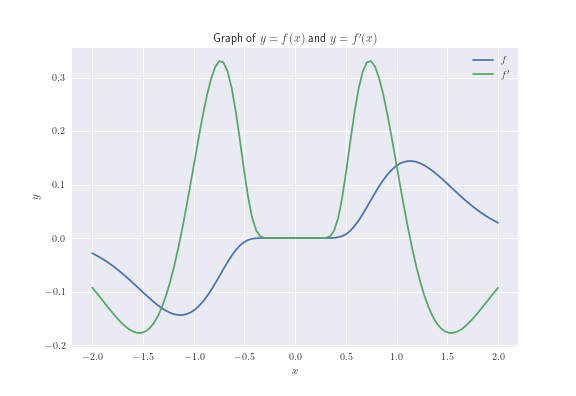
\includegraphics[scale = 0.4]{\pathtoimages/ex1-2.png}
\end{figure}

\end{frame}

\begin{frame}
\frametitle{Derivative Properties}
\begin{Theorem}
Suppose $\alpha$ and $\beta$ are constants and $f'$ and $g'$ exist. 
\begin{enumerate}
\item[(a)] $\displaystyle\frac{d}{dx}\left(\alpha f + \beta g\right) = \alpha f' + \beta g'$.
\item[(b)] $\displaystyle\frac{d}{dx}\left(f\cdot g\right) = g\cdot f' + f\cdot g'$
\item[(c)] $\displaystyle\frac{d}{dx}\left(\frac{f}{g}\right) = \frac{f'\cdot g - f\cdot g'}{g^2}$
\item[(d)] $\displaystyle\frac{d}{dx}\left(f\circ g\right) = \left(f' \circ g\right)\cdot g'$
\end{enumerate}
\end{Theorem}
\end{frame}

\begin{frame}
\frametitle{Useful Derivative Formulas}
Suppose $a > 0$.
\begin{multicols}{2}
\begin{itemize}
\item $\frac{d}{dx}(x^n) = n x^{n-1}$				
\item $\frac{d}{dx}(e^x)  = e^x$
\item $\frac{d}{dx}(a^x)  = a^x \ln a$
\item $\frac{d}{dx}\left(\ln|x|\right)  = \frac{1}{x},\ x\neq 0$
\item $\frac{d}{dx}\left(\log_a|x|\right) = \frac{1}{x\ln a},\ x\neq 0$
\item $\frac{d}{dx}\left(\sin x\right) = \cos x$
\item $\frac{d}{dx}\left(\cos x\right) = -\sin x$
\item $\frac{d}{dx}\left(\tan x\right) = \sec^2 x$
\item $\frac{d}{dx}\left(\arctan x\right) = \frac{1}{1 + x^2}$
\end{itemize}
\end{multicols}
\end{frame}

\begin{frame}[t]
\frametitle{Derivative Example}
\begin{Example}
$$
\frac{d}{dx}\left(e^{1/x}\sin x\right) = 
$$
\end{Example}

\end{frame}

\subsection{Tangent Lines}


\begin{frame}
\frametitle{Tangent Lines}
The tangent line of the graph of $y = f(x)$ at $(x_0, y_0)$ is
$$
y = y_0 + f'(x_0)(x - x_0).
$$
\end{frame}

\begin{frame}[t]
\frametitle{Tangent Line Example}
\begin{Example}
Approximate $\sqrt{3.9}$.
\end{Example}

\end{frame}


\subsection{Optimization}

\begin{frame}
\frametitle{Local and Global Extrema}

\begin{Definition}
Let $f$ be a function defined on domain $D$.\small
\begin{enumerate}
\item[(a)] The {\bf global maximum} of $f$ is at $c$ if $f(c)\geq f(x)$ for all $x$ in $D$. The {\bf global minimum} of $f$ is at $c$ if $f(c) \leq f(x)$ for all $x$ in $D$. The global maximum and global minimum values of $f$ are called the {\bf global extrema} of $f$.
\item[(b)] A {\bf local maximum} of $f$ is at $c$ if there is an interval $(a, b)$ such that $f(c) \geq f(x)$ for all $x$ in $(a, b)$ and $a < c < b$. Similarly, a {\bf local minimum} of $f$ is at $c$ there is an interval $(a, b)$ such that $f(c) \leq f(x)$ for all $x$ in $(a, b)$ and $a < c < b$. The local maximum and local minimum values of $f$ are called the {\bf local extrema} of $f$.
\end{enumerate}
\end{Definition}
\end{frame}

\begin{frame}
\frametitle{Local and Global Extrema Example}

\begin{figure}
\centering
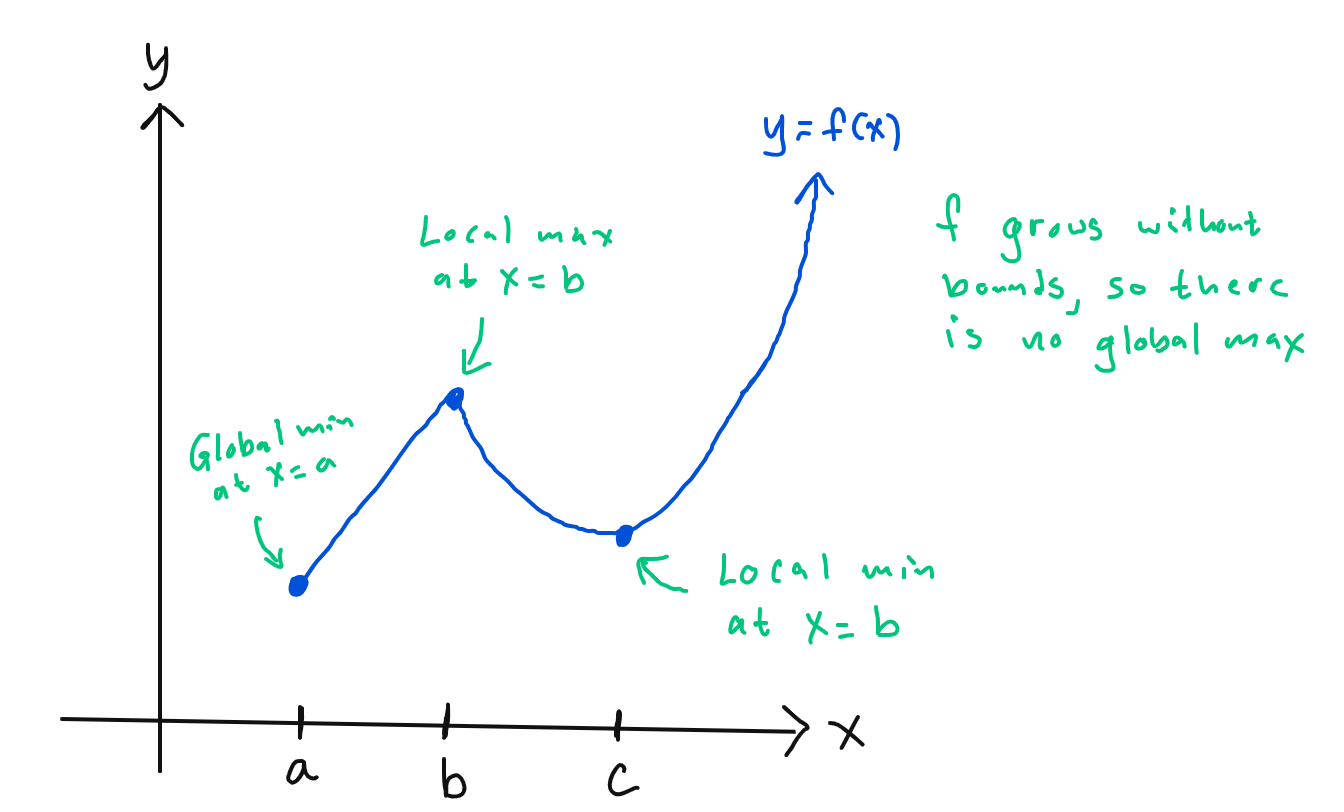
\includegraphics[scale = 0.4]{\pathtoimages/local-global.png}
\end{figure}



\end{frame}

\begin{frame}
\frametitle{Extreme Value Theorem}

\begin{Theorem}[Extreme Value Theorem]
If $f$ is continuous on a closed interval $[a, b]$, then $f$ attains a global maximum value $f(c)$ and a global minimum value $f(d)$ for some numbers $c$ and $d$ in $[a, b]$.
\end{Theorem}

\end{frame}

\begin{frame}[t]
\frametitle{Increasing and Decreasing Functions}
Assume f' exists.
\begin{itemize}
\item If $f'(x) > 0 $, then $f$ is increasing at $x$.
\item If $f' (x) < 0$, then $f$ is decreasing at $x$.
\end{itemize}

\end{frame}

\begin{frame}
\frametitle{First Derivative Test}
Suppose $x = c$ is a critical number, i.e. $c$ is in the domain of $f$ and $f'(c)$ is 0 or undefined.
\begin{itemize}
\item[(a)] If $f'$ changes from positive to negative at $x = c$, then $f$ has a local maximum at $x = c$.
\item[(b)] If $f'$ changes from negative to positive at $x = c$, then $f$ has a local minimum at $x = c$.
\item[(c)] If $f'$ does not change sign at $x = c$, then $f$ has no local extremum at $x = c$.
\end{itemize}
\end{frame}

\begin{frame}[t]
\frametitle{Optimization Example}
\small
\begin{Example}
Find the local and global extrema of the function $f(x) = x^3(x-2)^2$. Suppose the domain of $f$ is the closed interval $[-1, 3]$.
\end{Example}
\end{frame}

\begin{frame}
\frametitle{Second Derivative Test}
Suppose $f'(c) = 0$.
\begin{enumerate}
\item[(a)] If $f''(c) > 0$, then $f$ has a local minimum at $x = c$.
\item[(b)] If $f''(c) < 0$, then $f$ has a local maximum at $x = c$.
\item[(c)] If $f''(c) = 0$ or is undefined, then the test fails.
\end{enumerate}
\end{frame}

\begin{frame}[t]
\frametitle{Local Extrema Example}
\begin{Example}
Find all local extrema of $g(x) = x^4 - 4x^3$.
\end{Example}
\end{frame}


\subsection{L'H\^{o}pital's Rule}

\begin{frame}
\frametitle{L'H\^{o}pital's Rule}

\begin{Theorem}[L'H\^{o}pital's Rule]
Suppose the functions $f$ and $g$ are defined on the open interval $(a, b)$, $a < c < b$, $f$ and $g$ are differentiable on $(a, b)\setminus\{c\}$, and $g' (x) \neq 0$ for all $x$ in $(a, b)\setminus\{c\}$. If
$$
\lim_{x\to c} \frac{f'(x)}{g'(x)} = L
$$
and either
$$
\lim_{x\to c} f(x) = \lim_{x\to c} g(x) = 0\qquad\text{or}\qquad \lim_{x\to c} f(x) = \lim_{x\to c} g(x) = \infty,
$$
then
$$
\lim_{x\to c} \frac{f(x)}{g(x)} = L.
$$
\end{Theorem}
\end{frame}

\begin{frame}[t]
\frametitle{L'H\^{o}pital's Rule Cont.}
\begin{Example}
Prove $\displaystyle\lim_{x\to\infty} x^{1/x} = 1$.
\end{Example}
\end{frame}



\section{Integration}

\begin{frame}
\begin{center}
\Huge Integration
\end{center}
\end{frame}

\subsection{Riemann Integration}

\begin{frame}
\frametitle{Definite Integration}
\begin{center}
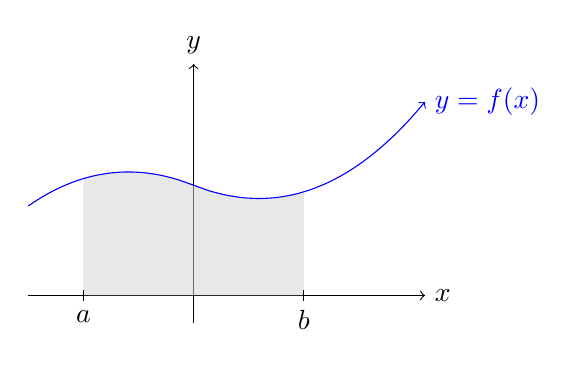
\begin{tikzpicture}[declare function = {f(\x) = 0.005 * \x^3 + 0.16 * \x^2 - 0.4 * \x + 2;}, scale = 0.7]
  \draw[->] (-3, 0) -- (4.2, 0) node[right] {$x$};
  \draw[->] (0, -0.5) -- (0, 4.2) node[above] {$y$};
  \fill [gray!35, domain=-2:2, variable=\x, opacity = 0.5]
  (-2, 0) -- plot ({\x}, {f(\x)}) -- (2, 0) -- cycle;
  
  \draw[->, domain=-3:4.2, smooth, variable= \x, blue] plot ({\x}, {f(\x)}) node[right] {$y = f(x)$};
  
  \draw (-2, 0.1) -- (-2, -0.1) node[below] {$a$};
  \draw (2, 0.1) -- (2, -0.1) node[below] {$b$};  
\end{tikzpicture}
\end{center}
The motivating problem for the definite integral is finding area under the graph $y = f(x)$ for $a \leq x \leq b$.
\end{frame}

\begin{frame}
\frametitle{Riemann Sum}
\begin{Definition}
Suppose we have a function $f$ defined on the interval $[a, b]$. Consider a {\bf partition pair} $P$ and $T$; $P = (x_0, x_1, \ldots x_n)$ and $T = (t_1, t_2, \ldots, t_n)$, where
$$
a = x_0 \leq t_1 \leq x_1 \leq \ldots\leq x_{n-1} \leq t_n \leq x_n = b.
$$ 
The {\bf Riemann sum} corresponding to the partition pair $P$ and $T$ is defined to be
$$
\sum_{k = 1}^n f(t_k)\Delta x_k.
$$
\end{Definition}
\end{frame}

\begin{frame}
\frametitle{Finer and Finer Partition}

\begin{center}
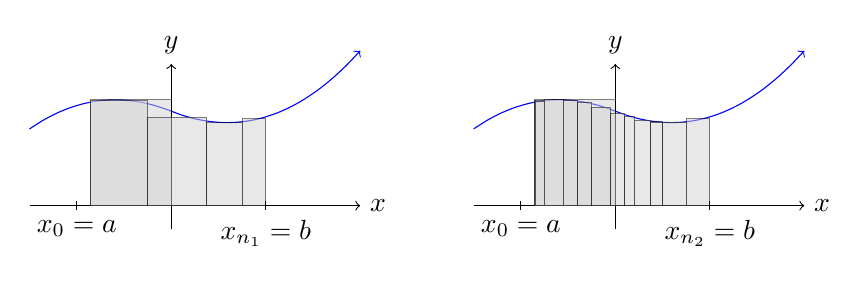
\begin{tikzpicture}[declare function = {f(\x) = 0.005 * \x^3 + 0.16 * \x^2 - 0.4 * \x + 2;}, scale = 0.6]

\def\offset{-4.7}

 \draw[->] ({-3 + \offset}, 0) -- ({4 + \offset}, 0) node[right] {$x$};
 \draw[->] ({0 + \offset}, -0.5) -- ({0 + \offset}, 3) node[above] {$y$};
  
  \draw[->, domain=-3:4, smooth, variable= \x, blue] plot ({\x + \offset}, {f(\x)});
  
  \def\lastx{-2}
  
	\foreach \x[count=\xi from 2, remember=\x as \lastx] in {-1.7, -0.5, 0.75, 1.5,  2} {
	\filldraw[color = black, fill = gray!35, opacity = 0.5] ({\lastx + \offset}, 0) -- ({\lastx +\offset}, {f(0.3 * \lastx + 0.7 * \x )}) -- ({\x + \offset}, {f(0.3 * \lastx + 0.7 * \x )}) -- ({\x + \offset}, 0) -- cycle;
}
      
  \draw ({-2 + \offset}, 0.1) -- ({-2 + \offset}, -0.1) node[below] {$x_0 = a$};
  \draw ({2 +\offset}, 0.1) -- ({2 + \offset}, -0.1) node[below] {$x_{n_1} = b$};  
  
\def\offset{4.7}

 \draw[->] ({-3 + \offset}, 0) -- ({4 + \offset}, 0) node[right] {$x$};
  \draw[->] ({0 + \offset}, -0.5) -- ({0 + \offset}, 3) node[above] {$y$};
  
  \draw[->, domain=-3:4, smooth, variable= \x, blue] plot ({\x + \offset}, {f(\x)});
  
  \def\lastx{-2}
  
	\foreach \x[count=\xi from 2, remember=\x as \lastx] in {-1.7, -1.5, -1.1, -0.8, -0.5, -0.1, 0.2, 0.4, 0.75, 1, 1.5,  2} {
	\filldraw[color = black, fill = gray!35, opacity = 0.5] ({\lastx + \offset}, 0) -- ({\lastx + \offset}, {f(0.3 * \lastx + 0.7 * \x )}) -- ({\x + \offset}, {f(0.3 * \lastx + 0.7 * \x )}) -- ({\x + \offset}, 0) -- cycle;
}
      
  \draw ({-2 + \offset}, 0.1) -- ({-2 + \offset}, -0.1) node[below] {$x_0 = a$};
  \draw ({2 +\offset}, 0.1) -- ({2 + \offset}, -0.1) node[below] {$x_{n_2} = b$};  
\end{tikzpicture}
\end{center}

The rectangles in the right figure do a better job of approximating the area under the curve. This is because the partition in the second figure is ``finer", i.e. uses more $x$-values, than the first.
\end{frame}

\begin{frame}
\frametitle{Partition Mesh}
\begin{Definition}
The {\bf mesh} of partition $P$ is
$$
\| P\| = \max\{\Delta x_1,\Delta x_2,\ldots \Delta x_n\}.
$$
\end{Definition}
As $\| P\| \to 0$, the approximation becomes better and better.
\end{frame}

\begin{frame}

\begin{Definition}
The {\bf Riemann integral} of $f$ over the interval $[a, b]$ is
$$
\int_a^b f(x)\ dx = \lim_{\|P\|\to 0} \sum_{k = 1}^n f(t_k) \Delta x_k
$$
whenever the limit converges. 
\end{Definition} 
\end{frame}

\begin{frame}
\frametitle{Integral Theorems}

\begin{Theorem}
A bounded function on an interval $[a, b]$ is Riemann integrable if it is continuous for all but a finite number of points. 
\end{Theorem}

\begin{Theorem}
If $f$ and $g$ are Riemann-integrable on $[a, b]$ and $\alpha$ and $\beta$ are constants, then the following hold.
\begin{enumerate}
\item[(a)] $\displaystyle \int_a^b \alpha f(x) + \beta g(x)\ dx = \alpha \int_a^b f(x)\ dx + \beta \int_a^b g(x)\ dx$
\item[(b)] $\displaystyle \int_a^b f(x)\ dx = \int_a^c f(x)\ dx + \int_c^b f(x)\ dx$ for any c in $[a, b]$
\end{enumerate}
\end{Theorem}
\end{frame}

\begin{frame}[t]
\frametitle{Analytic Example}
\small
\begin{Example}
Prove $\displaystyle\int_1^a \frac{dx}{x} = \ln a$ for $a > 1$. Use partition pairs of the form $P = (1, a^{1/n}, a^{2/n}\ldots, a)$ and $T = (1, a^{1/n}, a^{2/n}\ldots, a^{(n-1)/n})$.
\end{Example}
\end{frame}


\begin{frame}

\frametitle{Selection of $T$}
The most common choices for $T$ are
\begin{itemize}
\item Left endpoints:  $t_k = x_{k - 1}$
\item Midpoints: $t_k = \frac{x_{k - 1} + x_{k}}{2}$
\item Right endpoints: $t_k = x_{k}$
\end{itemize}

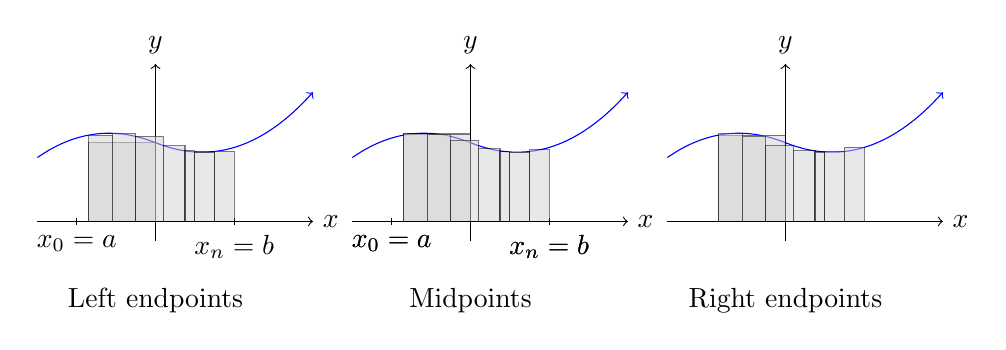
\begin{tikzpicture}[declare function = {f(\x) = 0.005 * \x^3 + 0.16 * \x^2 - 0.4 * \x + 2;}, scale = 0.5]

\def\offset{-8}

% Left endpoints
 \draw[->] ({-3 + \offset}, 0) -- ({4 + \offset}, 0) node[right] {$x$};
  \draw[->] (\offset, -0.5) -- (\offset, 4) node[above] {$y$};
  
  \draw[->, domain=-3:4, smooth, variable= \x, blue] plot ({\x + \offset}, {f(\x)});
  
  \def\lastx{-2}
  
	\foreach \x[count=\xi from 2, remember=\x as \lastx] in {-1.7, -1.1, -0.5, 0.2, 0.75, 1, 1.5,  2} {
	
	\filldraw[color = black, fill = gray!35, opacity = 0.5] ({\lastx + \offset}, 0) -- ({\lastx + \offset}, {f(\lastx)}) -- ({\x + \offset}, {f(\lastx)}) -- ({\x +\offset}, 0) -- cycle;
}
      
  \draw ({-2 + \offset}, 0.1) -- ({-2 + \offset}, -0.1) node[below] {$x_0 = a$};
  \draw ({2 + \offset}, 0.1) -- ({\offset + 2}, -0.1) node[below] {$x_n = b$};  
  
  \node at (\offset, -2) {Left endpoints};
  
    % Midpoints
  \def\offset{0}
  
  \draw[->] ({-3 + \offset}, 0) -- ({4 + \offset}, 0) node[right] {$x$};
  \draw[->] ({\offset}, -0.5) -- ({\offset}, 4) node[above] {$y$};
  
  \draw[->, domain=-3:4, smooth, variable= \x, blue] plot ({\x + \offset}, {f(\x)});
  
  \def\lastx{-2}
  
	\foreach \x[count=\xi from 2, remember=\x as \lastx] in {-1.7, -1.1, -0.5, 0.2, 0.75, 1, 1.5,  2} {
	\filldraw[color = black, fill = gray!35, opacity = 0.5] ({\lastx + \offset}, 0) -- ({\lastx + \offset}, {f(0.5 * \lastx + 0.5 * \x)}) -- ({\x + \offset}, {f(0.5 * \lastx + 0.5 * \x)}) -- ({\x +\offset}, 0) -- cycle;
}
      
  \draw ({-2 + \offset}, 0.1) -- ({-2 + \offset}, -0.1) node[below] {$x_0 = a$};
  \draw ({2 + \offset}, 0.1) -- ({2 + \offset}, -0.1) node[below] {$x_n = b$};  
  
      \node at (\offset, -2) {Midpoints};


 \def\offset{8}
  
  % Right endpoints
  \draw[->] ({-3 + \offset}, 0) -- ({4 + \offset}, 0) node[right] {$x$};
  \draw[->] ({\offset}, -0.5) -- ({\offset}, 4) node[above] {$y$};
  
  \draw[->, domain=-3:4, smooth, variable= \x, blue] plot ({\x + \offset}, {f(\x)});
  
  \def\lastx{-2}
  
	\foreach \x[count=\xi from 2, remember=\x as \lastx] in {-1.7, -1.1, -0.5, 0.2, 0.75, 1, 1.5,  2} {
	\filldraw[color = black, fill = gray!35, opacity = 0.5] ({\lastx + \offset}, 0) -- ({\lastx + \offset}, {f(\x)}) -- ({\x + \offset}, {f(\x)}) -- ({\x + \offset}, 0) -- cycle;
}
      
  \draw (-2, 0.1) -- (-2, -0.1) node[below] {$x_0 = a$};
  \draw (2, 0.1) -- (2, -0.1) node[below] {$x_n = b$};  
  
    \node at (\offset, -2) {Right endpoints};
    
 
\end{tikzpicture}

\end{frame}



\begin{frame}
\frametitle{Selection of $P$}
The most common choice for $P$, by far, is the uniform partition
$$
x_k = a + k \Delta x\qquad\text{and}\qquad \Delta x = \frac{b - a}{n}.
$$

\end{frame}

\begin{frame}
\frametitle{Useful formulas}
When working analytic problems with a uniform partition, these formulas come up a lot
$$
\sum_{k = 1}^n k = \frac{n(n + 1)}{2},\qquad \sum_{k = 1}^n k^2 = \frac{n(n+ 1)(2n+ 1)}{6}, 
$$
and
$$
\sum_{k = 1}^n k^3 = \frac{n^2(n+1)^2}{4} = \left[\frac{n(n+ 1)}{2}\right]^2.
$$
\end{frame}

\begin{frame}[t]
\frametitle{Uniform Partition Example}
\begin{Example}
Use uniform partitions and right endpoints to find $\displaystyle\int_0^1 x^2\ dx$.
\end{Example}
\end{frame}

\begin{frame}[fragile]
\frametitle{Python Code}

\begin{lstlisting}[language=Python]
# Define Riemann sum
def riemann_sum(f, P, pts):
    
    # Sort values
    P = np.sort(P)

    # Calculate Delta x
    dx_vals = np.diff(P) 

    # Define T
    if pts == 'left':

        T = P[:-1]

    elif pts == 'right':

        T = P[1:]

    elif pts == 'mid':
        
        T = (P[:-1] + P[1:])/2
        
    else:
        
        raise Exception('Currently only left, right, and midpoints are supported!')
        
    # Get area of rectangles; assumes f is vectorized
    rectangle_areas = f(T) * dx_vals
    
    # Return sum
    return np.sum(rectangle_areas)
\end{lstlisting}
\end{frame}

\begin{frame}
\frametitle{Improper Integral}
\begin{Definition}
{
\linespread{0.5}
\begin{enumerate}
\item[(a)] If the integrals exists for every $t \geq a$ and for every $s \leq b$, then
$$
\int_a^\infty f(x)\ dx = \lim_{t\to\infty}\int_a^t f(x)\ dx
$$
and
$$
\int_{-\infty}^b f(x)\ dx = \lim_{s\to-\infty}\int_s^b f(x)\ dx.
$$
\item[(b)] For any $c$ in $\mathbb{R}$, if both $\displaystyle\int_c^\infty f(x)\ dx$ and $\displaystyle\int_{-\infty}^c f(x)\ dx$ converge, then 
$$
\int_{-\infty}^\infty f(x)\ dx = \int_{-\infty}^c f(x)\ dx + \int_c^\infty f(x)\ dx.
$$
\end{enumerate}
}
\end{Definition}
\end{frame}

\begin{frame}[t]
\frametitle{Python Example}
\begin{Example}
Use \texttt{pandas} to create a data frame of Riemann sums with left endpoints, midpoints, and right endpoints, and uniform partitions to approximate $\displaystyle\int_0^\infty e^{-x^2/2}\ dx$. Consider $n = 10, 50, 100, 500,$ and 1000.
\end{Example}
\end{frame}

\begin{frame}[fragile]
\frametitle{Python Example Cont.}

{\bf Solution. } Since $e^{-x^2/2}$ goes to 0 rapidly, it's safe to use $b = 10$. 
\begin{lstlisting}[language=Python]
# Import pandas
import pandas as pd

# Define function
f = lambda x: np.e**(-x**2/2)

# Define the n-values
n_vals = [10, 50, 100, 500, 1000]

# Define the data frame
results = pd.DataFrame(index = n_vals, columns = ['left', 'mid', 'right'])

# Loop over values
for n in n_vals:
    
    # We can use np.linspace for a uniform partition
    partition = np.linspace(0, 10, n + 1)
    
    # Get left endpoint results
    results.loc[n, 'left'] = riemann_sum(f, partition, 'left')
    
    # Get midpoint results
    results.loc[n, 'mid'] = riemann_sum(f, partition, 'mid') 
 
    # Get right endpoint results
    results.loc[n, 'right'] = riemann_sum(f, partition, 'right')   

# Note: screenshot of output is ex1-3
results
\end{lstlisting}
\end{frame}

\begin{frame}[fragile]
\frametitle{Python Example Result}
The limit as $\| P\|\to 0$ is $\sqrt{\pi/2}\approx 1.253$.
\begin{center}
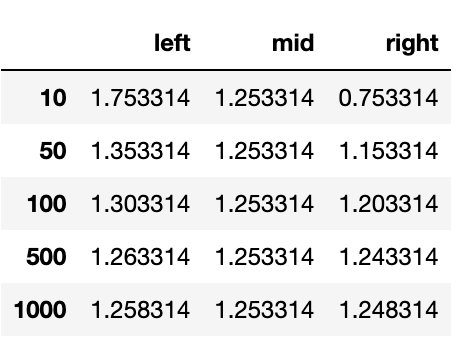
\includegraphics[scale = 0.8]{\pathtoimages/ex1-3.png}
\end{center}
\end{frame}

\subsection{Indefinite Integration} 


\begin{frame}
\frametitle{Indefinite Integral}

\begin{Definition}
The function $F$ is an {\bf indefinite integral} or {\bf antiderivative} of $f$ if $F'(x) = f(x)$. We write
$$
\int f(x)\ dx = F(x)
$$
to denote this.
\end{Definition}
Indefinite integrals are only unique up to a constant. For example, two antiderivatives of $2x$ are $x^2 +1$ and $x^2 - 4$. To handle all possibilities, we write
$$
\int 2x\ dx = x^2 + C.
$$
\end{frame}


\begin{frame}
\frametitle{Antiderivative Theorems}
\begin{Theorem}
Let $f$ and $g$ be continuous functions on some domain and let $\alpha$ and $\beta$ be real numbers. Then
$$
\int \alpha f(x) + \beta g(x)\ dx = \alpha \int f(x)\ dx + \beta \int g(x)\ dx.
$$
\end{Theorem}
\end{frame}

\begin{frame}
\frametitle{Useful Antiderivative Formulas}
\begin{multicols}{2}
{\small 
\begin{itemize}
\item $\displaystyle \int x^n\ dx = \frac{x^{n+ 1}}{n+ 1} + C$, $n\neq -1$
\item $\displaystyle \int \frac{dx}{x} = \ln|x| + C$	
\item $\displaystyle \int \frac{dx}{1 + x^2} = \arctan x + C$	
\item $\displaystyle \int e^x\ dx  = e^x + C$
\item $\displaystyle \int a^x\ dx = \frac{a^x}{\ln a} + C$
\item $\displaystyle\int \sin x\ dx = -\cos x + C$
\item $\displaystyle \int cos x\ dx= \sin x + C$
\item $\displaystyle\int \tan x\ dx = -\ln|cos x| + C$
\end{itemize}
}
\end{multicols}

\end{frame}

\begin{frame}
\frametitle{Fundamental Theorem of Calculus}

\begin{Theorem}[Fundamental Theorem of Calculus]
Suppose $f$ is continuous on the closed interval $[a, b]$. Then
\begin{enumerate}
\item[(a)] $\displaystyle\int_a^b f(x)\ dx = F(b) - F(a)$, where $F'(x)= f(x)$.
\item[(b)] $\displaystyle\frac{d}{dx}\left(\int_a^x f(t)\ tx\right) = f(x)$
\end{enumerate}
\end{Theorem}
\end{frame}

\begin{frame}[t]
\frametitle{Fundamental Theorem of Calculus Example}

\begin{Example}
$\displaystyle \int_0^2 \max\{x, 1\}\ dx = $
\end{Example}

\end{frame}

\begin{frame}
\frametitle{Proof of the Fundamental Theorem on YouTube}
Watch Peyam prove part (b) of the Fundamental Theorem of Calculus  (\url{https://youtu.be/4DrCKhCECHo}).
\begin{center}
\includegraphics[scale = 0.25]{\pathtoimages/peyam.png}
\end{center}
\end{frame}

\begin{frame}
\frametitle{u-Substitution} 

\begin{Theorem}[u-Substitution]
Suppose $g'$ is continuous on the closed interval $[a, b]$ and $f$ is continuous on the range of $g$. Then
$$
\int_a^b (f \circ g)(x)\cdot g'(x)\ dx = \int_{g(a)}^{g(b)} f(u)\ du.
$$
\end{Theorem}
\end{frame}

\begin{frame}[t]
\frametitle{Example}
\begin{Example}
$\displaystyle \int x e^{-x^2/2}\ dx =$
\end{Example}

\end{frame}

\begin{frame}
\frametitle{Integration by Parts}

\begin{Theorem}[Integration by parts]
Suppose $F$ and $G$ are differentiable functions, $F'(x) = f(x)$, and $G'(x) = g(x)$, where $f$ and $g$ are continuous. Then
$$
\int F(x) g(x)\ dx = F(x) G(x) - \int f(x) G(x)\ dx.
$$
\end{Theorem}
\end{frame}

\begin{frame}[t]
\frametitle{Example}
\begin{Example}
$\displaystyle\int \ln x\ dx = $
\end{Example}
\end{frame}

\section{Ordinary Differential Equations}

\begin{frame}
\begin{center}
\Huge Ordinary Differential Equations
\end{center}
\end{frame}

\begin{frame}
\frametitle{Ordinary Differential Equations}

\begin{Definition}
\begin{enumerate}
\item[(a)] An {\bf ordinary differential equation} (ODE) involves an unknown function of a single variable and some of its derivatives. 
\item[(b)] The {\bf order} of a differential equation is the order of the highest derivative that appears in the equation.
\end{enumerate}
\end{Definition} 
For example, $x y' = e^{xy}$ is a first order ordinary differential equation, while
$$
\frac{d^3 x}{dt^3} - 2t\dfrac{d^2x}{dt^2} + t^2 x = \cos t
$$
is a third order ordinary differential equation.

\end{frame}

\subsection{Separable ODEs}

\begin{frame}
\frametitle{Separable ODEs}
\begin{Definition}
An ODE of the form
$$
\frac{dy}{dx} = F(x, y)
$$
is separable if $F(x, y) = f(x) g(y)$.
\end{Definition}
It's relatively easy to solve separable differential equations 
$$
\frac{dy}{dx} =  f(x) g(y)\qquad\text{implies}\qquad \frac{1}{g(y)} \frac{dy}{dx}  = f(x).
$$
Hence,
$$
\int \frac{1}{g(y)} \frac{dy}{dx}\ dx = \int f(x)\ dx\qquad\text{implies}\qquad \int \frac{1}{g(y)}\ dy = \int f(x)\ dx.
$$
\end{frame}

\begin{frame}[t]
\frametitle{Separable ODE Example}
\small
\begin{Example}
Solve the differential equation
$$
\frac{dy}{dt} = \frac{ty + 3t}{t^2 + 1}
$$
subject to the initial condition $y(0) = 2$.
\end{Example}
\end{frame}

\subsection{First Order Linear ODEs}
\begin{frame}
\frametitle{Linear ODEs}
\begin{Definition}
A first order {\bf linear} differential equation is one that can be written in the form
$$
\frac{dy}{dx} + P(x) y = Q(x).
$$
\end{Definition}
The idea behind solving these is to find $\mu = f(x)$ such that
$$
\frac{d}{dx}\left(\mu y\right) = \mu \frac{dy}{dx} + \mu P(x) y.
$$
Using the product rule, it becomes clear
$$
\frac{d\mu}{dx} = \mu P(x)\qquad\text{implies}\qquad \mu = \exp\left(\int P(x)\ dx\right).
$$
\end{frame}

\begin{frame}[t]
\frametitle{Linear ODEs Example}
\small
\begin{Example}
Solve the differential equation 
$$
x\frac{dy}{dx} + 3x^3y = 6 x^3.
$$
\end{Example}
\end{frame}


\section{Sequences and Series}

\begin{frame}
\begin{center}
\Huge Sequences and Series
\end{center}
\end{frame}

\subsection{Sequences}

\begin{frame}
\frametitle{Sequences}
\begin{Definition}
A sequence $\displaystyle(a_n)_{n = 1}^\infty$ is said to {\bf converge}, if there is a value $a$ in $\mathbb{R}$ which has the property that: For all $\epsilon > 0$, there exists an integer $N$ such that $n\geq N$ implies that $|a_n - a| < \epsilon$.  We often write
$$
a_n\to a\qquad\text{or}\qquad\lim_{n\to\infty} a_n = a
$$
when $\displaystyle(a_n)_{n = 1}^\infty$ converges to $a$. If $\displaystyle(a_n)_{n = 1}^\infty$ does not converge, then it {\bf diverges}. 
\end{Definition}
\end{frame}

\begin{frame}[t]
\frametitle{Sequences Example}
\begin{Example}
Determine which of the following sequences converge/diverge. If the sequence converges, find its limit.
\begin{enumerate}
\item[(a)] $\displaystyle a_n = \frac{1}{n}$
\item[(b)] $\displaystyle b_n = \sqrt{n}$
\item[(c)]  $\displaystyle c_n = (-1)^n$
\item[(d)] $\displaystyle d_n = 1 + \frac{(-1)^n}{n}$
\end{enumerate} 
\end{Example}
\end{frame}

\begin{frame}[t]
\frametitle{Python Sequences Example}
\begin{Example}
Use Python to graph the four sequences in the previous example. Graph them on separate subplots, and for the sequences that converge use horizontal lines to show their respective limits.
\end{Example}

\end{frame}

\begin{frame}[fragile]
\frametitle{Python Sequences Example Solution}
\begin{multicols}{2}
\begin{lstlisting}[language=Python]

# Import modules 
import numpy as np
import matplotlib.pyplot as plt

# Use LaTeX
plt.rcParams['text.usetex'] = True

# Use Seaborn style
plt.style.use('seaborn')

# Define functions
a = lambda n: 1/n
b = lambda n: np.sqrt(n)
c = lambda n: (-1)**n
d = lambda n: 1 + (-1)**n/n

# Define the limits
a_lim, d_lim = 0, 1

# Get the n-values
n_vals = np.arange(1, 21)

# Get the sequence values
# Functions already vectorized
a_vals = a(n_vals)
b_vals = b(n_vals)
c_vals = c(n_vals)
d_vals = d(n_vals)

# Set up subplots
fig, ax = plt.subplots(2, 2, sharey = True, figsize = (10, 6))

# Plot a_n and its limit
ax[0, 0].scatter(n_vals, a_vals)
ax[0, 0].axhline(y = a_lim, color = 'r', linestyle = 'dashed')
ax[0, 0].set_xlabel(r'$n$')
ax[0, 0].set_ylabel(r'$a_n$')

# Plot b_n and its limit
ax[0, 1].scatter(n_vals, b_vals, label = r'$b_n$')
ax[0, 1].set_xlabel(r'$n$')
ax[0, 1].set_ylabel(r'$b_n$')

# Plot c_n and its limit
ax[1, 0].scatter(n_vals, c_vals)
ax[1, 0].set_xlabel(r'$n$')
ax[1, 0].set_ylabel(r'$c_n$')

# Plot d_n and its limit
ax[1, 1].scatter(n_vals, d_vals)
ax[1, 1].axhline(y = d_lim, color = 'r', linestyle = 'dashed')
ax[1, 1].set_xlabel(r'$n$')
ax[1, 1].set_ylabel(r'$d_n$')

plt.suptitle(r'Sequence Plots')

# Save the figure
plt.savefig(path + r'ex1-4.png')

plt.show()
\end{lstlisting}
\end{multicols}
\end{frame}

\begin{frame}
\frametitle{Python Sequences Example Result}
\begin{center}
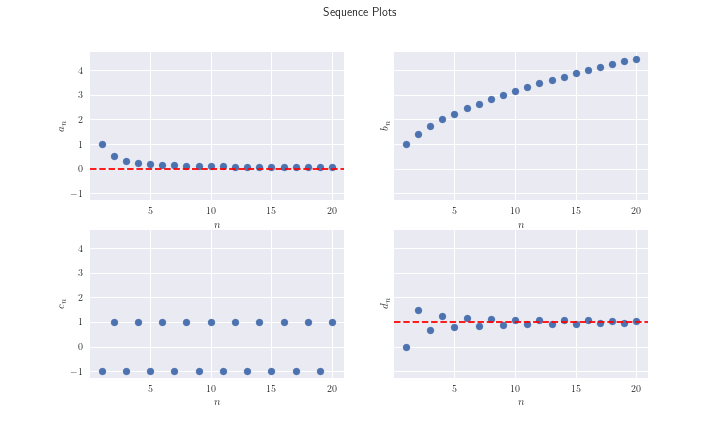
\includegraphics[scale = 0.4]{\pathtoimages/ex1-4.png}
\end{center}
\end{frame}

\begin{frame}
\frametitle{Triangle Inequality}
For any real numbers $x$, $y$, and $z$,
$$
|x - y| \leq |x -z| + |z - y|.
$$
\end{frame}

\frame{
\frametitle{Sequences}
\begin{Theorem}
\begin{itemize}
\item[(a)] The sequence $\displaystyle(a_n)_{n = 1}^\infty$ converges to $a$ in  $\mathbb{R}$ if and only if for every $\epsilon > 0$, we have $a_n$ in the interval $(a - \epsilon, a + \epsilon)$ for all but finitely many $n$.
\item[(b)] If $\displaystyle(a_n)_{n = 1}^\infty$ converges to both $a$ and $b$, then $a = b$.
\item[(c)] If $\displaystyle(a_n)_{n = 1}^\infty$ converges, then it is bounded. That is, convergence of $\displaystyle(a_n)_{n = 1}^\infty$ implies there exists a real number $B$ such that $|a_n| \leq B$ for all $n$.
\end{itemize}
\end{Theorem}
}

\frame{
\frametitle{Sequence Properties} 
\begin{Theorem} 
Suppose $\displaystyle(a_n)_{n = 1}^\infty$ and $\displaystyle(b_n)_{n = 1}^\infty$ are real numbered sequences and
$$
\lim_{n\to\infty} a_n = a\qquad\text{and}\qquad\lim_{n\to\infty} b_n = b.
$$
Let $\alpha$ and $\beta$ be real constants.
\begin{enumerate}
\item[(a)] $\displaystyle\lim_{n\to\infty}\left(\alpha a_n + \beta b_n\right) = \alpha a + \beta b$
\item[(b)] $\displaystyle\lim_{n\to\infty} a_n b_n = ab$
\item[(c)] $\displaystyle\lim_{n\to\infty} \frac{1}{a_n} = \frac{1}{a}$ if $a_n \neq 0$ and $a\neq 0$.
\end{enumerate}
\end{Theorem}
}

\begin{frame}
\frametitle{Monotonic Sequences}

\begin{Definition}
\begin{itemize}
\item A real sequence $(a_n)_{n = 1}^\infty$ is {\bf monotonically increasing} if $a_n \leq a_{n + 1}$ for all $n$.
\item A real sequence $(a_n)_{n = 1}^\infty$ is {\bf monotonically decreasing} if $a_n \geq a_{n + 1}$ for all $n$.
\end{itemize}
\end{Definition}

\begin{Theorem}
Suppose that  $(a_n)_{n = 1}^\infty$ is monotonic. Then it converges if and only if it is bounded.
\end{Theorem}
\end{frame}

\subsection{Series}

\begin{frame}
\frametitle{Series}
\begin{Definition}
Consider a series $\displaystyle S = \sum_{k = 1}^\infty a_k$. Its {\bf $\boldsymbol n$-th partial sum} is $\displaystyle S_n = \sum_{k = 1}^n a_k$. The series $S$ {\bf converges} if the sequence $(S_n)_{n = 1}^\infty$ converges, and it {\bf diverges} otherwise.
 \end{Definition}
 \end{frame}
 
 \begin{frame}[t]
 \frametitle{Example}
 \begin{Example}
 For what values of $r$ does the geometric series $\displaystyle\sum_{k = 1}^\infty r^{k - 1}$ converge?
 \end{Example}
 \end{frame}
 
 \begin{frame}
 \frametitle{Geometric Series}
 The geometric series is extremely important in finance. Remember these formulas. 
 $$
 \sum_{k= 1}^n a r^{k -1} = \frac{a(1 - r^n)}{1 - r}
 $$
 and
 $$
  \sum_{k = 1}^\infty a r^{k -1} =\begin{cases} \frac{a}{1 - r}, & |r| < 1\\ DNE,	& |r| \geq 1\end{cases}
 $$
  \end{frame}
  
  \begin{frame}
  \frametitle{Partial Fraction Decomposition}
\begin{itemize}
\item $\dfrac{a x + b}{(x - c)(x - d)} = \dfrac{A}{x - c} + \dfrac{B}{x - d},\quad c \neq d.$
\item $\dfrac{ax + b}{(x - c)^2} = \dfrac{A}{x - c} + \dfrac{B}{(x - c)^2}.$
\end{itemize}
  \end{frame}
  
 \begin{frame}[t]
 \frametitle{Partial Fraction Decomposition Example}
 \begin{Example}
Rewrite $\dfrac{x - 2}{x(x - 3)}$ using partial fraction decomposition.
 \end{Example}

  \end{frame}
  
  \begin{frame}[t]
   \frametitle{Convergent Series}
   \begin{Example}
   Show $\displaystyle\sum_{k = 1}^\infty \frac{1}{k(k + 1)}$ converges. 
   \end{Example}
  
  \end{frame}
 
 \begin{frame}
 \frametitle{Divergence Test}
 \begin{itemize}
\item If $\displaystyle\lim_{k\to\infty} a_k \neq 0$, then $\displaystyle\sum_{k = 1}^\infty a_k$ diverges.  
\item If $\displaystyle\lim_{k\to\infty} a_k =  0$, then $\displaystyle\sum_{k = 1}^\infty a_k$ may or may not converge.
\end{itemize}
 \end{frame}
 
 \begin{frame}
 \frametitle{Property of Series}
 
 \begin{Theorem} 
 Suppose that $\displaystyle\sum_{k = 1}^\infty a_k$ and $\displaystyle\sum_{k = 1}^\infty b_k$ converge. For any real constants $\alpha$ and $\beta$
 $$
 \sum_{k = 1}^\infty\left( \alpha a_k + \beta b_k\right) =   \alpha \sum_{k = 1}^\infty a_k + \beta \sum_{k = 1}^\infty b_k .
 $$
  \end{Theorem} 
 \end{frame}
 
 
 \begin{frame}
 \frametitle{Dominating Series}
 
 \begin{Theorem}
 If a series $\displaystyle\sum_{k = 1}^\infty b_k$ dominates a series $\displaystyle\sum_{k = 1}^\infty a_k$ in the sense that for all sufficiently large $k$, $|a_k| \leq b_k$, then convergence of $\displaystyle\sum_{k = 1}^\infty b_k$ implies convergence of $\displaystyle\sum_{k = 1}^\infty a_k$.
 \end{Theorem}
 
 \end{frame}
 
 \begin{frame}[t]
  \frametitle{Dominating Series Example}
  \begin{Example} 
  Show that the series $\displaystyle\sum_{k = 1}^\infty \frac{\sin k}{2^k}$ converges.
  \end{Example}
 
 \end{frame}
 
 \begin{frame}
  \frametitle{Integral Test}
  
  \begin{Theorem}[Integral Test]
 Suppose $f$ is continuous and $f(k) = a_k$.
\begin{enumerate}
\item[(a)] If $|a_k| \leq f(x)$ for all sufficiently large $k$ and all $x$ in the interval $(k - 1, k]$, then convergence of $\displaystyle\int_1^\infty f(x)\ dx$ implies convergence of $\displaystyle\sum_{k = 1}^\infty a_k$.
\item[(b)] If $|f(x)| \leq a_k$ for all sufficiently large $k$ and all $x$ in the interval $[k, k+1)$ then diverges of $\displaystyle\int_1^\infty f(x)\ dx$ implies divergence of $\displaystyle\sum_{k = 1}^\infty a_k$.
\end{enumerate}
\end{Theorem}
  
  \end{frame}
  
  \begin{frame}[t]
  \frametitle{Example (p-Series)}
  \begin{Example}
  Prove that $\displaystyle\sum_{k = 1}^\infty \frac{1}{k^p}$ converges for $p > 1$ and diverges for $p\leq 1$.
  \end{Example}
  
  \end{frame}
  
  \begin{frame}
  \frametitle{Alternating Series Test}
  
  \begin{Theorem} 
Suppose the alternating series $\displaystyle\sum_{k = 1}^\infty (-1)^{k + 1} b_k$ is such that $0 \leq b_{k + 1} \leq b_k$ for sufficiently large $k$. Then the series converges if $\displaystyle\lim_{n\to\infty} b_k = 0$.
  \end{Theorem}
  \end{frame}
   
  \begin{frame}[t]
 \frametitle{Alternating Series Test Example}
 \begin{Example}
 Show that the series $\displaystyle\sum_{k = 1}^\infty \frac{(-1)^{k + 1}}{k}$ converges.
 \end{Example}
 
 \end{frame}
 
 
 \begin{frame}
  \frametitle{Absolutely and Conditionally Convergent Series}
  
  \begin{Definition}
  A series $\displaystyle\sum_{k = 1}^\infty a_k$ is {\bf absolutely convergent} if $\displaystyle\sum_{k = 1}^\infty |a_k|$ converges. A series is {\bf conditionally convergent} if $\displaystyle\sum_{k = 1}^\infty a_k$ converges but $\displaystyle\sum_{k = 1}^\infty |a_k|$ does not.
  \end{Definition}
  For example, the series
  $$
  \sum_{k = 1}^\infty \frac{(-1)^{k + 1}}{k}
  $$
  is conditionally convergent but not absolutely. 
  
 \end{frame}
 
 \begin{frame}
   \frametitle{Ratio Test}
   \begin{Theorem}
   \begin{enumerate}
   \item[(a)] If $\displaystyle\lim_{k\to\infty} \left|\frac{a_{k + 1}}{a_k}\right| = L < 1$, then the series $\displaystyle\sum_{k = 1}^\infty a_k$ is absolutely convergent.
   \item[(b)] If $\displaystyle\lim_{n\to\infty}\left|\frac{a_{k + 1}}{a_k}\right| = L > 1$, then the series $\displaystyle\sum_{k = 1}^\infty a_k$  is divergent.
   \item[(c)] If $\displaystyle\lim_{n\to\infty}\left|\frac{a_{k + 1}}{a_k}\right| = L = 1$, then the test fails.
   \end{enumerate}
   \end{Theorem}
 \end{frame}
 
 \begin{frame}[t]
  \frametitle{Ratio Test Example} 
  \begin{Example}
What can be said about the convergence of $\displaystyle\sum_{k = 1}^\infty (-1)^k\frac{k!}{k^k}$?
\end{Example}
\end{frame}

\subsection{Power Series}

\begin{frame}
\frametitle{Power Series}
\begin{Definition}
A {\bf power series} centered at $c$ is a series of the form
$$
\sum_{k = 0}^\infty a_k (x - c)^k.
$$
If the series converges for $|x - c| < R$ and diverges for $|x - c| > R$, then $R$ is the {\bf radius of convergence}. The {\bf interval of convergence} $I$ is the set of all $x$ values where the series converges. 
\end{Definition}
{\bf Remark:} We assume $0^0 = 1$ within our power series, so the power series always converges at $x = c$.
\end{frame}

\begin{frame}[t]
\frametitle{Power Series Example}
\begin{Example}
Find the radius and interval of convergence of the series $\displaystyle\sum_{k = 0}^\infty \frac{(-3)^k (x + 1)^k}{\sqrt{k + 1}}$.
\end{Example}

\end{frame}

\begin{frame}
\frametitle{Differentiation and Integration of Power Series}
\begin{Theorem}
If the power series $f(x) = \displaystyle\sum_{k = 0}^\infty a_k (x - c)^k$ has radius of convergence $R > 0$, then both
\begin{enumerate}
\item[(a)] $\displaystyle f'(x) = \sum_{k = 1}^\infty k a_k (x - c)^{k - 1}$ and
\item[(b)] $\displaystyle\int f(x)\ dx = C + \sum_{k = 0}^\infty a_k \frac{(x - c)^{k + 1}}{k + 1}$
\end{enumerate}
have radii of convergence $R$.
\end{Theorem}
\end{frame}

\begin{frame}[t]
\frametitle{Differentiation of Power Series Example}
\begin{Example}
$\displaystyle\sum_{k = 1}^\infty \frac{k}{1.10^k}$ = 
\end{Example}
\end{frame}

\begin{frame}
\frametitle{Taylor's Theorem}
\begin{Theorem}
Suppose
$$
f(x) = \sum_{k = 0}^\infty a_k (x - c)^k\qquad\text{for}\qquad |x - c| < R.
$$
Then
$$
a_k = \frac{f\ ^{(k)}(c)}{k!}.
$$
\end{Theorem}
\end{frame}

\begin{frame}
\frametitle{Popular Taylor Series Centered at Zero}
%\begin{multicols}{2}
{\small
\begin{itemize}
\item $\displaystyle \frac{1}{1 - x} = \sum_{k = 0}^\infty x^k$ for $x\in (-1, 1)$
\item $\displaystyle e^x = \sum_{k = 0}^\infty \frac{x^k}{k!}$ for $x\in\mathbb{R}$
\item $\displaystyle\sin x = \sum_{k = 0}^\infty (-1)^k \frac{x^{2k +1}}{(2k + 1)!}$ for $x\in\mathbb{R}$
\item $\displaystyle\cos x = \sum_{k = 0}^\infty (-1)^k \frac{x^{2k}}{(2k)!}$ for $x\in\mathbb{R}$
\item $\displaystyle\arctan x = \sum_{k = 0}^\infty (-1)^k \frac{x^{2k + 1}}{2k+ 1}$ for $x\in [-1, 1]$
\end{itemize}
}
%\end{multicols}

\end{frame}

\begin{frame}[t]
\frametitle{Taylor's Theorem Example}
\begin{Example}
Prove $\displaystyle\arctan x = \sum_{k = 0}^\infty (-1)^k \frac{x^{2k + 1}}{2k+ 1}$ for $x\in [-1, 1]$.
\end{Example}
\end{frame}

\section{Time Value of Money}

\begin{frame}
\begin{center}
\Huge Time Value of Money
\end{center}
\end{frame}

\begin{frame}
\frametitle{Time Value of Money}

For a time $t$ cash flow $C_t$ discounted at rate $r$, the {\it present value} is
$$
PV = \frac{C_t}{(1 + r)^t}.
$$
The time $T$ {\it future value} is
$$
FV_T = PV\cdot (1 + r)^T = C_t\cdot (1 + r)^{T- t}.
$$
\end{frame}

\begin{frame}
\frametitle{Compound Interest}
\small 
We assumed that interest is compounded once per unit of time. However, if it is compounded $n$ times per unit of time the formulas become
$$
PV = \frac{C_t}{\left(1 + \frac{r}{n}\right)^{nt}}\qquad\text{and}\qquad FV_T = PV\cdot \left(1 + \frac{r}{n}\right)^{nT}.
$$
Since
$$
\lim_{n\to\infty} \left(1 + \frac{r}{n}\right)^{nt} = e^{rt}
$$
for continuous compounding (i.e. $n = \infty$) the formulas are
$$
PV = C_t e^{-rt} \qquad\text{and}\qquad FV_T = PV\cdot  e^{rT} = C_t\cdot  e^{r(T - t)}
$$
\end{frame}

\begin{frame}
\frametitle{Multiple Cash Flows} 
Suppose we have a sequence of cash flows $C_0, C_1, C_2,\ldots, C_T$, where the subscript denotes the time of the cash flow, the {\it net present value} (NPV) of these cash flows discounted at the constant rate $r$ is
$$
NPV = C_0 + \frac{C_1}{1 + r} + \frac{C_2}{(1 + r)^2} + \ldots + \frac{C_n}{(1 + r)^T}.
$$
\end{frame}

\begin{frame}[t]
\frametitle{Time Value of Money Python Example}
\small
\begin{Example}
\begin{center}
\begin{tabular}{| l | c c c c c |}
\hline
Time			&	0		&	1	&	2	&	3	&	4\\\hline
Cash Flow	&	-100		&	50	&	20	&	70	&	10\\\hline
\end{tabular}
\end{center}
Calculate the net present value given a continuously compounded discount rate of 5\%.
\end{Example}
\end{frame}

\begin{frame}[fragile]
\frametitle{Time Value of Money Python Solution}
\begin{lstlisting}[language=Python]
# Import module
import numpy as np

# Record rate
rate = 0.05

# Record time of cash flows
time = np.array([0, 1, 2, 3, 4])

# Record cash flows
cash_flows = np.array([-100, 50, 20, 70, 10])

# Get the NPV
NPV = np.sum(cash_flows * np.exp(-rate * time))

print(f'The NPV of the cash flows is {NPV:.2f}.')
\end{lstlisting}

$NPV \approx 34.10$
\end{frame}

\begin{frame}
\frametitle{\texttt{numpy\_finance} Module}

There is a \texttt{numpy\_finance} module that has a net present value function (\url{https://numpy.org/numpy-financial/latest/npv.html}). However, we would need the annual rate to use it in the last example, i.e. we would have to use the rate 
$$
100\% \times (e^{0.05} - 1) \approx 5.127\%.
$$
\end{frame}

\begin{frame}[t]
\frametitle{Time Value of Money Example}
\small
\begin{Example}
Jain borrows \$1,000,000 to purchase a house. The loan is for thirty years and her first payment is one month from when she initially borrows the money. If her annualized rate is 12\%, what will be her monthly payments? Ignore fees.
\end{Example}

\end{frame}

\begin{frame}
\frametitle{Growing Payments}
Suppose 1 is payed at time $1$, and payments increase at a rate of $g$ each subsequent period until a final payment of $(1 + g)^{n -1}$ is made at time $n$. If cash flows are discounted at rate $r$, then the NPV of the cash flows is
$$
\frac{1 - \left(\frac{1 + g}{1 + r}\right)^n}{r - g}.
$$
\end{frame}

\begin{frame}[t]
\frametitle{Growing Payments Example}
\tiny
\begin{Example}
Calculate the NPV of the series of end-of-year cash flows. Assume 
\begin{itemize}
\item \$100 is payed in the first year,
\item each subsequent year payments increase by 5\%, 
\item the final payment is made at the end of year ten, and
\item the discount rate is 8\%.
\end{itemize} 
\end{Example}

\end{frame}

\end{document}
